\section*{(12\textordfeminine\ aula) --- Como testar a MQ: ensembles, valores médios e variáveis compatíveis}

\subsection*{Como testar a MQ?}

O colapso do vetor de estado após uma medida ideal é a ferramenta usada para se preparar estados quânticos específicos e se testar as predições da teoria (em uma partícula em um estado desconhecido).

Se ao medir $\hat{R}$ obtemos como resultado um autovalor \textbf{NÃO DEGENERADO}, o postulado III diz que o estado da partícula passa a ser o autovetor associado (unicamente definido, a menos de uma constante multiplicativa). Se o resultado da medida for um autovalor \textbf{DEGENERADO}, sabemos apenas que o estado, após a medida, está no subespaço degenerado; para especificar o estado temos que fazer uma medida de \textbf{OUTRO OBSERVÁVEL} cujo operador comute com $\hat{R}$ (verdadeiramente).

\begin{center}
\begin{tikzpicture}[scale=1]

    \draw[->,thick] (0,0) -- (0,1.6) node[above] {$\ket{\omega_1}$};
    \draw[->] (0,0) -- (1.8,0) node[right] {$\ket{\omega_2,1}$};
    \draw[->] (0,0) -- (-1.2,-1.2) node[below left] {$\ket{\omega_2,2}$};
    \node at (0,-2) {\footnotesize resultado após medir $\hat{R}$ e obter $\omega_1$};

    \begin{scope}[xshift=6.5cm]
        \draw[->,thick] (0,0) -- (0,1.6) node[above] {$\ket{\omega_1}$};
        \draw[->] (0,0) -- (1.8,0.5) node[right] {$\ket{\omega_2,1}$};
        \draw[->] (0,0) -- (-1.2,-1.2) node[below left] {$\ket{\omega_2,2}$};
        \draw[dashed,->] (-0.3,0.9) -- (0.6,0.25) node[midway, above] {\footnotesize ?};
        \node at (0,-2) {\footnotesize resultado após medir $\hat{R}$ e obter $\omega_2$};
    \end{scope}
\end{tikzpicture}
\end{center}

\noindent (no caso da direita: o autovalor $\omega_1$ é não degenerado, mas $\omega_2$ é degenerado, com o subespaço gerado por $\ket{\omega_2,1}$ e $\ket{\omega_2,2}$; o operador que vai especificar o estado dentro desse subespaço deve comutar com $\hat{R}$.)

\subsection*{Ensemble quântico}

Um conjunto de $N$ partículas no \textbf{MESMO ESTADO} $\ket{\Psi}$ se chama um \textbf{ENSEMBLE QUÂNTICO}.

Se $\ket{\Psi}$ é conhecido você pode fazer previsões sobre a distribuição de resultados experimentais.

\textbf{Exemplo:}
\begin{equation}
    \ket{\Psi} = \sum_{i=1}^{6} c_i \ket{\omega_i} \qquad \text{(base ortonormal de autovetores de $\hat{R}$, normalizado, } \sum_{i=1}^{6}|c_i|^2 = 1 \text{)}
\label{eq:aula12_estado_ensemble}
\end{equation}

Fazendo medidas de $\hat{R}$ em um ensemble de $N$ partículas no estado $\ket{\Psi}$ acima você terá (no limite $N\to\infty$)
\begin{equation}
    \begin{cases}
        N|c_1|^2 \text{ resultados } \omega_1 \\
        N|c_2|^2 \text{ \quad ''\ \ } \omega_2 \\
        \quad \vdots \\
        N|c_6|^2 \text{ \quad ''\ \ } \omega_6
    \end{cases}
\label{eq:aula12_ocorrencias}
\end{equation}
onde $N|c_i|^2$ é o número de ocorrências do resultado $\omega_i$.

A média dos $N$ resultados é
\begin{equation}
    \frac{1}{N}\sum_i \underbrace{N|c_i|^2}_{\text{\# ocorrências}} \omega_i = \sum_i |c_i|^2 \omega_i
\label{eq:aula12_media_ocorrencias}
\end{equation}

Não podemos prever o resultado de uma medida em particular, mas podemos prever a \textbf{MÉDIA} dos $N$ resultados (no limite $N\to\infty$).

\begin{center}
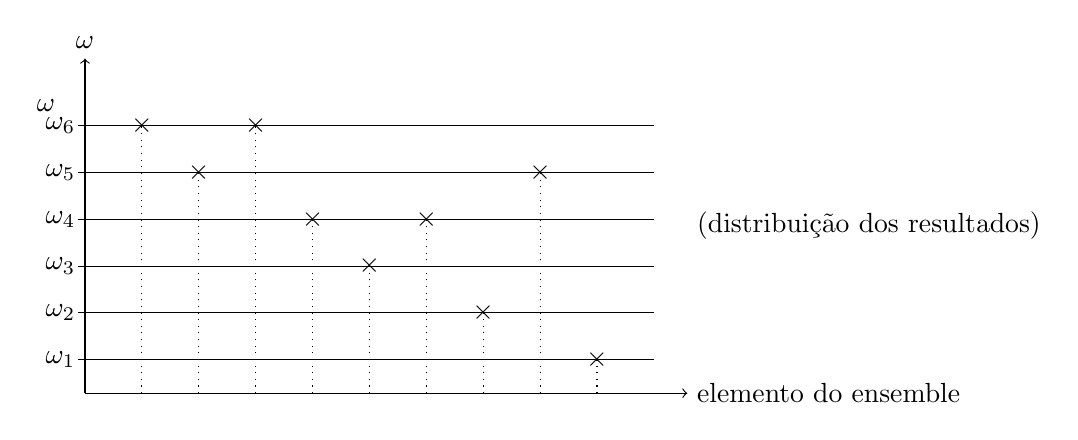
\begin{tikzpicture}[scale=0.85]
    \draw[->] (0,0) -- (9,0) node[right] {elemento do ensemble};
    \draw[->] (0,0) -- (0,5) node[above] {$\omega$};
    \foreach \y/\lab in {0.5/\omega_1, 1.2/\omega_2, 1.9/\omega_3, 2.6/\omega_4, 3.3/\omega_5, 4.0/\omega_6}{
        \draw (-0.1,\y) -- (8.5,\y);
        \node[left] at (0,\y) {$\lab$};
    }
    \node[anchor=east] at (-0.3,4.3) {$\omega$};
    \foreach \x/\y in {1/4.0, 2/3.3, 3/4.0, 4/2.6, 5/1.9, 6/2.6, 7/1.2, 8/3.3, 9/0.5}{
        \node at (\x*0.85,\y) {$\times$};
        \draw[dotted] (\x*0.85,0) -- (\x*0.85,\y);
    }
    \node[right] at (9,2.5) {(distribuição dos resultados)};
\end{tikzpicture}
\end{center}

\subsection*{Valor esperado ou valor médio (espectro discreto)}

A média dos resultados experimentais pode ser prevista:
\begin{align}
    \aver{R} &= \sum_i \underbrace{P(\omega_i)}_{\text{probabilidade}} \underbrace{\omega_i}_{\text{resultado}} \notag\\
    &= \sum_i \braket{\Psi}{\hat{P}_{\omega_i}}{\Psi}\, \omega_i \qquad \text{(supondo } \braket{\Psi}{\Psi}=1 \text{, usando expressão de } \hat{P}_{\omega_i}\text{)} \notag \\
    &= \sum_i \sum_\alpha |\bra{\Psi}\ket{\omega_i,\alpha}|^2\, \omega_i \qquad (\alpha \to \text{autovalor}) \label{eq:aula12_valor_medio_1}
\end{align}

Lembrando que $\hat{R}\ket{\omega_i,\alpha} = \omega_i\ket{\omega_i,\alpha}$,
\begin{equation}
    \aver{R} = \sum_i \sum_\alpha \braket{\Psi}{\hat{R}}{\omega_i,\alpha}\braket{\omega_i,\alpha}{\Psi} \qquad \left(\text{usando } \sum_{i,\alpha} \ket{\omega_i,\alpha}\bra{\omega_i,\alpha} = \hat{\mathbb{1}}\right)
\label{eq:aula12_valor_medio_2}
\end{equation}

\begin{equation}
    \boxed{\aver{R} = \matrixel{\Psi}{\hat{R}}{\Psi}}
\label{eq:aula12_valor_medio_final}
\end{equation}

A expressão \eqref{eq:aula12_valor_medio_1} é conveniente quando $\ket{\Psi}$ já está expresso na base de autovetores de $\hat{R}$, e a expressão \eqref{eq:aula12_valor_medio_final} nos demais casos (quando $\ket{\Psi}$ é conhecido em uma base genérica do EV).

\textbf{Ex:} $\ket{\Psi} = \dfrac{1}{\sqrt{2}}\ket{\omega_1} + \dfrac{1}{2}\ket{\omega_2} + \dfrac{1}{2}\ket{\omega_3}$ (normalizado)
\begin{equation}
    \aver{R} = \frac{1}{2}\omega_1 + \frac{1}{4}\omega_2 + \frac{1}{4}\omega_3
\label{eq:aula12_exemplo_discreto}
\end{equation}

Se (em um EV de dimensão 3, com $\ket{1}, \ket{2}, \ket{3}$ como base):
\begin{equation}
    \ket{\Psi} = \frac{1}{\sqrt{2}}\ket{1} + \frac{1}{\sqrt{2}}\ket{2} \qquad \text{(normalizado)}
\label{eq:aula12_exemplo_base_generica}
\end{equation}

\noindent \textbf{Obs:} O EV da MQ é de dimensão infinita, quase nunca escreveremos operadores como matriz. No caso 1D teremos
\begin{equation}
    \matrixel{\Psi}{\hat{R}}{\Psi} = \int_{-\infty}^{\infty}\int_{-\infty}^{\infty} dx\, dx' \; \braket{\Psi}{x}\matrixel{x}{\hat{R}}{x'}\braket{x'}{\Psi}
\label{eq:aula12_R_continuo}
\end{equation}

e
\begin{equation}
    \hat{R} \leftrightarrow
    \begin{pmatrix}
        1 & 0 & 1 \\
        0 & 1 & 0 \\
        1 & 0 & 2
    \end{pmatrix}
    \qquad \text{(Hermitiana)}
\label{eq:aula12_matriz_R}
\end{equation}

\begin{equation}
    \matrixel{\Psi}{\hat{R}}{\Psi} = \sum_{i=1}^{3}\sum_{j=1}^{3} \braket{\Psi}{i}\matrixel{i}{\hat{R}}{j}\braket{j}{\Psi}
\label{eq:aula12_R_soma_matricial}
\end{equation}

em forma matricial:
\begin{equation}
    \begin{pmatrix} \psi_1^* & \psi_2^* & \psi_3^* \end{pmatrix}
    \begin{pmatrix} \hat{R} \end{pmatrix}
    \begin{pmatrix} \psi_1 \\ \psi_2 \\ \psi_3 \end{pmatrix}
\label{eq:aula12_R_matricial_geral}
\end{equation}

\begin{equation}
    = \begin{pmatrix} \dfrac{1}{\sqrt{2}} & \dfrac{1}{\sqrt{2}} & 0 \end{pmatrix}
    \begin{pmatrix} 1 & 0 & 1 \\ 0 & 1 & 0 \\ 1 & 0 & 2 \end{pmatrix}
    \begin{pmatrix} 1/\sqrt{2} \\ 1/\sqrt{2} \\ 0 \end{pmatrix}
\label{eq:aula12_R_matricial_exemplo}
\end{equation}

\begin{equation}
    = \begin{pmatrix} 1/\sqrt{2} & 1/\sqrt{2} & 0 \end{pmatrix}
    \begin{pmatrix} 1/\sqrt{2} \\ 1/\sqrt{2} \\ 1/\sqrt{2} \end{pmatrix}
    = \frac{1}{2} + \frac{1}{2} + 0 = \boxed{1}
\label{eq:aula12_R_matricial_resultado}
\end{equation}

\subsection*{Variância (desvio padrão) ou incerteza (espectro discreto)}

A distribuição dos resultados em torno da média pode também ser prevista:
\begin{equation}
    \Delta R = \sqrt{\aver{(\hat{R} - \aver{R})^2}}
\label{eq:aula12_def_incerteza}
\end{equation}

O termo que está sendo promediado é o quadrado da diferença entre o resultado da medida $R$ e o valor médio $\aver{R}$.

\textbf{Exemplo.} Na turma as notas foram $\{5, 10, 8, 7, 8\}$.

Qual a nota média?
\begin{equation}
    \frac{1}{5}(5+10+8+7+8) = \boxed{7{,}6} = \aver{N}
\label{eq:aula12_nota_media}
\end{equation}

Qual o desvio padrão (ao quadrado)?
\begin{align}
    &\frac{1}{5}\Big[(5-7{,}6)^2 + (10-7{,}6)^2 + (8-7{,}6)^2 + (7-7{,}6)^2 + (8-7{,}6)^2\Big] \notag \\
    &= \boxed{2{,}64} = (\Delta N)^2
\label{eq:aula12_desvio_notas}
\end{align}

\begin{equation}
    (\Delta N)^2 = \frac{1}{N}\sum_{i=1}^{N}(N_i - \aver{N})^2 = \frac{1}{N}\sum_{i=1}^{N}\left(N_i^2 - 2N_i\aver{N} + \aver{N}^2\right) = \aver{N^2} - \aver{N}^2
\label{eq:aula12_desvio_expandido}
\end{equation}

onde $\aver{N^2} = \dfrac{1}{N}\sum_i N_i^2$ e $\aver{N} = \dfrac{1}{N}\sum_i N_i$.

No nosso caso:
\begin{equation}
    \aver{N^2} = \frac{1}{5}\left(5^2+10^2+8^2+7^2+8^2\right) = 60{,}4
\label{eq:aula12_N2_medio}
\end{equation}

\begin{equation}
    \aver{N}^2 = 57{,}76 \qquad \left(\Rightarrow (\Delta N)^2 = 60{,}4 - 57{,}76 = 2{,}64\right)
\label{eq:aula12_N_medio_quadrado}
\end{equation}

$\Delta N = \sqrt{2{,}64} = 1{,}6$ informa a faixa \textbf{EM TORNO DA MÉDIA} onde as notas se distribuem.

\begin{center}
\begin{tikzpicture}[scale=1]
    \draw[->] (0,0) -- (7,0) node[right] {(aluno) $n$};
    \draw[->] (0,0) -- (0,3) node[above] {nota};
    \draw[thick] (0.3,1.6) -- (6.5,1.6) node[right,xshift=-3mm] {};
    \node[left] at (0,1.6) {$\aver{N}$};
    \draw[dashed] (0.3,2.0) -- (6.5,2.0);
    \draw[dashed] (0.3,1.2) -- (6.5,1.2);
    \draw[<->] (1.0,1.6) -- (1.0,2.0) node[midway,right] {$\Delta N$};
    \foreach \x/\y in {0.6/2.3,1.1/1.0,1.6/2.0,2.1/1.5,2.6/1.9,3.1/1.4,3.6/1.7,4.1/1.3,4.6/2.1,5.1/1.6,5.6/1.2,6.1/1.8}{
        \node[circle,fill=black,inner sep=1pt] at (\x,\y) {};
    }
\end{tikzpicture}
\end{center}

Assim,
\begin{equation}
    \boxed{(\Delta R)^2 = \aver{R^2} - \aver{R}^2}
\label{eq:aula12_formula_geral_variancia}
\end{equation}
onde $\aver{R^2} = \matrixel{\Psi}{\hat{R}^2}{\Psi}$ e $\aver{R} = \matrixel{\Psi}{\hat{R}}{\Psi}$ (supondo $\braket{\Psi}{\Psi}=1$).

\textbf{Exemplo.}
\begin{equation}
    \ket{\Psi} = \frac{1}{\sqrt{2}}\ket{\omega{=}1} + \frac{1}{2}\ket{\omega{=}{-}1} + \frac{1}{2}\ket{\omega{=}2} \qquad \text{(normalizado)}
\label{eq:aula12_exemplo_variancia_estado}
\end{equation}

\begin{equation}
    \aver{R} = \frac{1}{2}(1) + \frac{1}{4}(-1) + \frac{1}{4}(2) = \frac{3}{4} = \boxed{0{,}75}
\label{eq:aula12_exemplo_R_medio}
\end{equation}

\begin{equation}
    \aver{R^2} = \frac{1}{2}(1)^2 + \frac{1}{4}(-1)^2 + \frac{1}{4}(2)^2 = \frac{7}{4} = \boxed{1{,}75}
\label{eq:aula12_exemplo_R2_medio}
\end{equation}

\begin{equation}
    \Delta R = \sqrt{1{,}75 - 0{,}75^2} = \boxed{1{,}09}
\label{eq:aula12_exemplo_deltaR}
\end{equation}

Assim como no cálculo de $\aver{R}$, é conveniente ter $\ket{\Psi}$ expresso em termos dos autovetores de $\hat{R}$:
\begin{align}
    \aver{R^2} &= \sum_{i,\alpha} \matrixel{\Psi}{\hat{R}^2}{\omega_i,\alpha}\braket{\omega_i,\alpha}{\Psi} \notag \\
    &= \sum_{i,\alpha} \omega_i^2 \braket{\Psi}{\omega_i,\alpha}\braket{\omega_i,\alpha}{\Psi} \notag \\
    &= \sum_{i,\alpha} \omega_i^2 \,\big|\braket{\Psi}{\omega_i,\alpha}\big|^2 \qquad \text{(coeficiente da expansão ao quadrado)}
\label{eq:aula12_R2_expansao}
\end{align}
onde usei que $\ket{\omega_i,\alpha}$ é autovetor de \textbf{QUALQUER POTÊNCIA} do operador $\hat{R}$.

\textbf{Obs.} A incerteza é nula, $\Delta R = 0$, quando $\ket{\Psi}$ é uma combinação linear de autovetores de $\hat{R}$ de \textbf{MESMO AUTOVALOR}. Nesse caso $\hat{R}\ket{\Psi} = \omega\ket{\Psi}$ e $\hat{R}^2\ket{\Psi} = \omega^2\ket{\Psi}$.

Isso faz com que $\matrixel{\Psi}{\hat{R}}{\Psi} = \omega$ e $\matrixel{\Psi}{\hat{R}^2}{\Psi} = \omega^2$
\begin{equation}
    \Delta R^2 = \omega^2 - \omega^2 = 0
\label{eq:aula12_deltaR_nula}
\end{equation}

\textbf{TODAS AS MEDIDAS PRODUZEM $\omega$ COMO RESULTADO!}

\begin{center}
\begin{tabular}{c|c}
    \textbf{EXPERIMENTO} & \textbf{CÁLCULO} \\
    \hline
    $\dfrac{1}{N}(\omega_1+\omega_2+\cdots+\omega_N) \;(=\overline{\omega})$ & $\matrixel{\Psi}{\hat{R}}{\Psi}$ \\[3mm]
    $\dfrac{1}{N}\left[(\omega_1-\overline{\omega})^2+(\omega_2-\overline{\omega})^2+\cdots+(\omega_N-\overline{\omega})^2\right]$ & $\matrixel{\Psi}{\hat{R}^2}{\Psi} - \matrixel{\Psi}{\hat{R}}{\Psi}^2$ \\
    $(=\Delta\omega^2)$ &
\end{tabular}
\end{center}

\fbox{\parbox{0.92\textwidth}{
\textbf{VERIFIQUE SEMPRE} se seu cálculo de $\aver{R}$ é um valor entre o maior e o menor autovalor presente em $\ket{\Psi}$. (Mas, em geral, $\aver{R}$ \textbf{NÃO} é um dos autovalores!)
}}

\subsection*{Variáveis compatíveis e incompatíveis}

Duas variáveis são \textbf{COMPATÍVEIS} quando seus operadores comutam. Nesse caso existem autovetores comuns a ambos operadores.

A medida em sequência de operadores compatíveis é a maneira de se preparar um estado quântico bem definido (ver a observação do início da aula).

Suponha que medimos $\hat{R}$ em um estado desconhecido e obtivemos $\omega_2$, um autovalor degenerado.
\begin{equation}
    \ket{?} \xrightarrow{\;\hat{R}\;} \ket{\omega_2}
\label{eq:aula12_medida_degenerada}
\end{equation}

O estado $\ket{\omega_2}$ não é definido, sabemos apenas que ele está no subespaço do autovalor $\omega_2$.

Outra medida de $\hat{R}$ não adianta, pois o estado já é um autovetor de $\hat{R}$ e não será alterado pela medida (postulado III).

\begin{center}
\begin{tikzpicture}[scale=1]
    \draw[->,thick] (0,0) -- (0,1.8) node[above] {$\ket{\omega_1}=\ket{\lambda_1}$};
    \draw[->] (0,0) -- (2.0,0.3) node[right] {$\ket{\omega_2,1}$};
    \draw[->] (0,0) -- (-1.0,-1.0) node[below] {$\ket{\lambda_3}$};
    \draw[->] (0,0) -- (1.0,-1.0) node[below] {$\ket{\lambda_2}$};
    \draw[->] (0,0) -- (-2.0,0.3) node[left] {$\ket{\omega_2,2}$};
\end{tikzpicture}
\end{center}

Se $\hat{A}$ e $\hat{R}$ comutam, seus autovetores são comuns. Na figura os autovetores de $\hat{A}$ são não degenerados.

Note que
\begin{equation}
    \hat{R}\ket{\lambda_1} = \omega_1\ket{\lambda_1}, \qquad \hat{R}\ket{\lambda_2} = \omega_2\ket{\lambda_2}, \qquad \hat{R}\ket{\lambda_3} = \omega_2\ket{\lambda_3}
\label{eq:aula12_autovetores_comuns}
\end{equation}
($\ket{\lambda_2}$ e $\ket{\lambda_3}$ estão no subespaço $\omega_2$).

Uma medida de $\hat{A}$ no estado indeterminado $\ket{\omega_2}$ vai produzir $\ket{\lambda_2}$ ou $\ket{\lambda_3}$, um estado determinado.
\begin{equation}
    \ket{\omega_2} \xrightarrow{\;\hat{A}\;}
    \begin{cases}
        \ket{\omega_2,\lambda_2} \\
        \ket{\omega_2,\lambda_3}
    \end{cases}
\label{eq:aula12_medida_A_apos_R}
\end{equation}

\fbox{\parbox{0.92\textwidth}{
\textbf{Um CONJUNTO COMPLETO DE OBSERVÁVEIS QUE COMUTAM} é um conjunto de operadores que comutam (portanto com autovetores comuns) e que especificam \textbf{UNICAMENTE} um estado com a informação dos autovalores.

Um único operador com autovalores \textbf{NÃO degenerados} tem essa propriedade.

Dois operadores com autovalores \textbf{degenerados} têm essa propriedade se, dentro do subespaço degenerado de $\hat{R}$, os autovalores de $\hat{A}$ são \textbf{DISTINTOS}.
}}

\begin{equation}
    \boxed{\text{Se } \ket{\omega,\lambda} \text{ é estado único} \;\Leftrightarrow\; \hat{R} \text{ e } \hat{A} \text{ são C.C.O.C.}}
\label{eq:aula12_ccoc}
\end{equation}

\subsection*{Sequência de medidas}

\textbf{(i)} $[\hat{R}, \hat{A}] = 0$

\begin{equation}
    \ket{\Psi} \xrightarrow{\;\hat{R}\;} \ket{\omega_1} \xrightarrow{\;\hat{A}\;} \ket{\lambda_1} = \ket{\omega_1,\lambda_1}
\label{eq:aula12_sequencia_compativel}
\end{equation}

\begin{center}
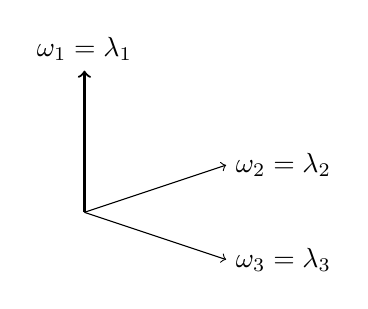
\begin{tikzpicture}[scale=1]
    \draw[->,thick] (0,0) -- (0,1.8) node[above] {$\ket{\omega_1}=\ket{\lambda_1}$};
    \draw[->] (0,0) -- (1.8,0.6) node[right] {$\ket{\omega_2}=\ket{\lambda_2}$};
    \draw[->] (0,0) -- (1.8,-0.6) node[right] {$\ket{\omega_3}=\ket{\lambda_3}$};
\end{tikzpicture}
\end{center}

O estado $\ket{\lambda_1}$ é um autoestado de $\hat{A}$ \textbf{DENTRO DO} subespaço do autovalor $\omega_1$, portanto qualquer medida de $\hat{R}$ ou $\hat{A}$ após essas 2 medidas irá dar sempre $\omega_1$ ou $\lambda_1$.

\textbf{(ii)} $[\hat{R}, \hat{A}] \neq 0$ (não há autovetores comuns)

\begin{center}
\begin{tikzpicture}[scale=1]
    \draw[->,thick] (0,0) -- (0,1.8) node[above] {$\ket{\omega_3}$};
    \draw[->] (0,0) -- (1.8,0.5) node[right] {$\ket{\omega_2}$};
    \draw[->] (0,0) -- (1.4,-1.3) node[right] {$\ket{\omega_1}$};
    \draw[->] (0,0) -- (-1.6,0.7) node[left] {$\ket{\lambda_2}$};
    \draw[->] (0,0) -- (-1.0,-1.5) node[left] {$\ket{\lambda_1}$};
\end{tikzpicture}
\end{center}

\begin{equation}
    \ket{\Psi} \xrightarrow{\;\hat{R}\;} \ket{\omega_1} \xrightarrow{\;\hat{A}\;} \ket{\lambda_2}
\label{eq:aula12_sequencia_incompativel}
\end{equation}

O vetor $\ket{\lambda_2}$ \textbf{NÃO É AUTOVETOR} de $\hat{R}$, medida de $\hat{R}$ nesse estado pode dar qualquer resultado $\{\omega_1, \omega_2, \omega_3\}$.

O caso clássico de variáveis que não comutam é o dos operadores posição $\hat{X}$ e momentum $\hat{P} = \hbar\hat{K}$
\begin{equation}
    [\hat{X}, \hat{P}] = i\hbar
\label{eq:aula12_comutador_XP}
\end{equation}

Não há autovetores simultâneos, não existe um estado quântico que produza uma posição bem definida (seja autovetor de $\hat{X}$) \textbf{E} um momentum bem definido (seja autovetor de $\hat{P}$).

\noindent\textbf{Obs:} Mesmo quando 2 operadores \textbf{NÃO COMUTAM}, $[\hat{R},\hat{A}] = \hat{\Sigma}$, onde $\hat{\Sigma}$ é um operador não nulo, ainda podemos encontrar um \textbf{NÚMERO LIMITADO} de autovetores comuns de $\hat{R}$ e $\hat{A}$. Isso pode acontecer caso o operador $\hat{\Sigma}$ tenha autovalores nulos. Suponha que $\ket{\omega\lambda}$, um autovetor comum, exista
\begin{align}
    \hat{R}\hat{A}\ket{\omega\lambda} &= \hat{R}\,\lambda\ket{\omega\lambda} = \lambda\omega\ket{\omega\lambda} \notag \\
    \hat{A}\hat{R}\ket{\omega\lambda} &= \hat{A}\,\omega\ket{\omega\lambda} = \lambda\omega\ket{\omega\lambda}
\label{eq:aula12_autovetor_comum_naocomutam}
\end{align}
subtraindo,
\begin{equation}
    [\hat{R},\hat{A}]\ket{\omega\lambda} = 0 \;\Rightarrow\; \hat{\Sigma}\ket{\omega\lambda} = 0
\label{eq:aula12_subtraindo_comutador}
\end{equation}

O autovetor comum é autovetor de $\hat{\Sigma}$ com autovalor nulo! No caso $[\hat{X},\hat{P}] = i\hbar$ isso não ocorre, pois $(i\hbar)\hat{\mathbb{1}} = \hat{\Sigma}$ não tem autovalor nulo.

\subsection*{Valores médios de operadores de espectro contínuo}

\textbf{Exemplo 4.2.4} --- Seja uma partícula no estado
\begin{equation}
    \ket{\Psi} = \int_{-\infty}^{\infty} dx \, \ket{x}\braket{x}{\Psi}
\label{eq:aula12_estado_continuo}
\end{equation}
onde a função de onda $\braket{x}{\Psi} = \Psi(x) = A \exp\left[-(x-a)^2/2\Delta^2\right]$ (essa função se chama \textbf{Gaussiana}).

\begin{center}
\begin{tikzpicture}[scale=1]
    \draw[->] (-0.5,0) -- (6,0) node[right] {$x$};
    \draw[->] (0,0) -- (0,2.5) node[above] {$\Psi(x)$};
    \draw[scale=1, domain=-0.5:6, smooth, variable=\x, thick] plot ({\x},{2*exp(-((\x-3)*(\x-3))/2.2)});
    \draw[<->] (2.3,1.7) -- (3.7,1.7) node[midway,above] {$\Delta$};
    \node[below] at (3,0) {$a$};
\end{tikzpicture}
\end{center}

\noindent\textbf{Normalizando} $\ket{\Psi}$ (trata-se de um vetor próprio):
\begin{align}
    \braket{\Psi}{\Psi} &= \int_{-\infty}^{\infty} dx \, \braket{\Psi}{x}\braket{x}{\Psi} = 1 \notag \\
    &= A^2 \int_{-\infty}^{\infty} dx\, e^{-(x-a)^2/\Delta^2} = A^2\sqrt{\pi\Delta^2} \;\Rightarrow\; \boxed{A = \frac{1}{(\pi\Delta^2)^{1/4}}}
\label{eq:aula12_normalizacao_gaussiana}
\end{align}

\fbox{\parbox{0.92\textwidth}{
\textbf{Integral de Gaussiana:}
\begin{equation}
    \int_{-\infty}^{\infty} e^{-\alpha x^2}\, dx = \sqrt{\frac{\pi}{\alpha}}
\label{eq:aula12_integral_gaussiana}
\end{equation}
}}

A função de onda normalizada é
\begin{equation}
    \Psi(x) = \frac{1}{(\pi\Delta^2)^{1/4}}\, e^{-(x-a)^2/2\Delta^2}
\label{eq:aula12_psi_normalizada}
\end{equation}

A probabilidade de encontrar a partícula entre $[x_1,x_2]$:
\begin{equation}
    P([x_1,x_2]) = \int_{x_1}^{x_2} dx \, |\braket{x}{\Psi}|^2 = \int_{x_1}^{x_2} \frac{1}{\sqrt{\pi\Delta^2}}\, e^{-(x-a)^2/\Delta^2}\, dx
\label{eq:aula12_probabilidade_intervalo}
\end{equation}

\noindent (projetor da medida: $\displaystyle \hat{P}([x_1,x_2]) = \int_{x_1}^{x_2} dx\, \ket{x}\bra{x}$)

\bigskip
\noindent\textbf{*} Aqui estou imaginando que a "largura natural do aparelho de medida" é infinitesimal.

Uma série de medidas de posição nesse estado tem como média dos resultados experimentais:
\begin{equation}
    \aver{X} = \matrixel{\Psi}{\hat{X}}{\Psi} = \int_{-\infty}^{\infty} dx \, \underbrace{\braket{\Psi}{x}}_{\Psi^*(x)}\underbrace{\braket{x}{\hat{X}}{\Psi}}_{x\,\Psi(x)}
\label{eq:aula12_X_medio_def}
\end{equation}

\begin{equation}
    = \int_{-\infty}^{\infty} dx\; \underbrace{x}_{\text{resultado}}\, \underbrace{|\Psi(x)|^2}_{\text{dens. prob.}}
\label{eq:aula12_X_medio_integral}
\end{equation}

\noindent\textbf{Obs:} Essa é a versão contínua de $\displaystyle\sum_i \omega_i P(\omega_i) = \aver{R}$.

\begin{equation}
    = \int_{-\infty}^{\infty} dx\; x\, \frac{1}{\sqrt{\pi\Delta^2}}\, e^{-(x-a)^2/\Delta^2}
    = \int_{-\infty}^{\infty} dy\; (y+a)\, \frac{1}{\sqrt{\pi\Delta^2}}\, e^{-y^2/\Delta^2} = a \qquad (y = x-a)
\label{eq:aula12_X_medio_calculo}
\end{equation}

\begin{equation}
    \boxed{\aver{X} = a} \qquad \text{(dimensão de comprimento)}
\label{eq:aula12_X_medio_resultado}
\end{equation}

O desvio padrão em torno desse valor médio é dado por
\begin{equation}
    \Delta X = \sqrt{\aver{X^2} - \aver{X}^2} = \sqrt{\aver{X^2} - a^2}
\label{eq:aula12_deltaX_def}
\end{equation}

\begin{equation}
    \aver{X^2} = \matrixel{\Psi}{\hat{X}\hat{X}}{\Psi} = \int_{-\infty}^{\infty} dx\; \underbrace{\braket{\Psi}{x}}_{\Psi^*(x)}\underbrace{\braket{x}{\hat{X}\hat{X}}{\Psi}}_{x^2\Psi(x)}
\label{eq:aula12_X2_medio_def}
\end{equation}

\begin{equation}
    = \int_{-\infty}^{\infty} dx\; x^2\, \frac{1}{\sqrt{\pi\Delta^2}}\, e^{-(x-a)^2/\Delta^2}
    = \int_{-\infty}^{\infty} dy\; (y^2+2ya+a^2)\, \frac{e^{-y^2/\Delta^2}}{\sqrt{\pi\Delta^2}} \qquad (y=x-a)
\label{eq:aula12_X2_medio_calculo}
\end{equation}

\begin{equation}
    = \Delta^2/2 + a^2 \qquad \text{(dimensão de } [L]^2 \text{)}
\label{eq:aula12_X2_medio_resultado}
\end{equation}

\fbox{\parbox{0.92\textwidth}{
\textbf{Integral de Gaussianas e potências:}
\begin{align}
    \int_{-\infty}^{\infty} dx\; x\, e^{-\alpha x^2} &= 0 \qquad \text{(pois o integrando é ímpar)} \label{eq:aula12_int_gauss_x1} \\
    \int_{-\infty}^{\infty} dx\; x^2\, e^{-\alpha x^2} &= -\frac{d}{d\alpha}\left[\int_{-\infty}^{\infty} dx\, e^{-\alpha x^2}\right] = -\frac{d}{d\alpha}\left(\sqrt{\frac{\pi}{\alpha}}\right) = \frac{\sqrt{\pi}}{2\alpha^{3/2}} \label{eq:aula12_int_gauss_x2} \\
    \int_{-\infty}^{\infty} dx\; x^4\, e^{-\alpha x^2} &= \frac{d^2}{d\alpha^2}\left[\int_{-\infty}^{\infty} dx\, e^{-\alpha x^2}\right] = \frac{3}{4}\frac{\sqrt{\pi}}{\alpha^{5/2}}, \quad \text{etc.} \label{eq:aula12_int_gauss_x4}
\end{align}
}}

Portanto $\boxed{\Delta X = \dfrac{\Delta}{\sqrt{2}}}$ (dimensão de $[L]$).

Uma série de medidas de momentum nesse estado tem como média dos resultados experimentais:
\begin{equation}
    \aver{P} = \matrixel{\Psi}{\hat{P}}{\Psi} = \int_{-\infty}^{\infty} dx\; \underbrace{\braket{\Psi}{x}}_{\Psi^*(x)}\underbrace{\braket{x}{\hat{P}}{\Psi}}_{-i\hbar \frac{d\Psi}{dx}}
\label{eq:aula12_P_medio_def}
\end{equation}

\begin{equation}
    = -i\hbar \int_{-\infty}^{\infty} dx\; \Psi(x)\frac{d\Psi}{dx} = -\frac{i\hbar}{2}\int_{-\infty}^{\infty} \frac{d}{dx}\left[\Psi^2(x)\right] dx
\label{eq:aula12_P_medio_integral}
\end{equation}

\begin{equation}
    = -\frac{i\hbar}{2}\Big[\Psi^2(\infty) - \Psi^2(-\infty)\Big] = 0 \qquad (\Rightarrow \text{ver Ex. 4.2.2})
\label{eq:aula12_P_medio_resultado}
\end{equation}

Para calcular o desvio padrão dos resultados:
\begin{equation}
    \aver{P^2} = \int_{-\infty}^{\infty} dx\; \underbrace{\braket{\Psi}{x}}_{\Psi^*(x)}\underbrace{\braket{x}{\hat{P}\hat{P}}{\Psi}}_{-\hbar^2 \frac{d^2}{dx^2}\Psi(x)} = \frac{\hbar^2}{2\Delta^2} \qquad \text{(dimensão } [\text{momento}]^2 \text{)}
\label{eq:aula12_P2_medio}
\end{equation}

(faça a conta, é importante praticar com essas integrais Gaussianas!)

Portanto $\boxed{\Delta P = \dfrac{\hbar}{\sqrt{2}\,\Delta}}$ (dimensão momentum).

\noindent\textbf{Obs:} A dimensão de $\Delta X$ deve ser \textbf{DISTÂNCIA} e a dimensão de $\Delta P$ deve ser \textbf{MOMENTUM}!

A amplitude de probabilidade associada à medida de $P$ é (isso é a "função de onda na representação $p$")
\begin{equation}
    \braket{p}{\Psi} = \int_{-\infty}^{\infty} dx\; \underbrace{\braket{p}{x}}_{\Psi_p^*(x)}\underbrace{\braket{x}{\Psi}}_{\Psi(x)}
\label{eq:aula12_p_psi_def}
\end{equation}

Quem é $\Psi_p(x) = \braket{x}{p}$, a autofunção do operador $\hat{P}$?
\begin{equation}
    \hat{P}\ket{p} = p\ket{p} \quad (\text{\# real}) \;\Rightarrow\; \matrixel{x}{\hat{P}}{p} = p\braket{x}{p}
\label{eq:aula12_autofuncao_P_def}
\end{equation}

Como em geral acontece, a equação de autovetores vira uma EDO.
\begin{equation}
    -i\hbar \frac{d\Psi_p}{dx} = p\,\Psi_p(x) \;\Rightarrow\; \Psi_p(x) = A\, e^{ipx/\hbar}
\label{eq:aula12_edo_autofuncao_P}
\end{equation}

Claramente é um vetor impróprio, como o $\ket{k}$ da seção 1.10. Escolhemos $A = \dfrac{1}{\sqrt{2\pi\hbar}}$ para obter a normalização de delta de Dirac.
\begin{equation}
    \braket{p}{p'} = \int_{-\infty}^{\infty} dx\, \Psi_p^*(x)\Psi_{p'}(x) = A^2\int_{-\infty}^{\infty} dx\, e^{i(p'-p)x/\hbar} = \underbrace{2\pi\,\delta\!\left(\frac{p'-p}{\hbar}\right)}_{} = \delta(p-p')
\label{eq:aula12_normalizacao_p}
\end{equation}

Usando $\delta\!\left(\dfrac{p-p'}{\hbar}\right) = \hbar\,\delta(p-p')$ (lembre do Exercício 1.10.1)
\begin{equation}
    \Rightarrow \boxed{A^2 = \frac{1}{2\pi\hbar}}
\label{eq:aula12_A2_resultado}
\end{equation}

\begin{equation}
    \braket{x}{p} = \frac{1}{\sqrt{2\pi\hbar}}\, e^{ipx/\hbar}
\label{eq:aula12_braket_xp}
\end{equation}

é uma função de onda (imprópria) de momentum bem definido (igual a $p$).

\begin{equation}
    \braket{x}{a} = \delta(x-a)
\label{eq:aula12_braket_xa}
\end{equation}
é uma função de onda (imprópria) de posição bem definida (igual a $a$).

\subsection*{Finalmente}

\begin{equation}
    \braket{p}{\Psi} = \int_{-\infty}^{\infty} dx\; \frac{1}{\sqrt{2\pi\hbar}}\, e^{-ipx/\hbar}\; \frac{1}{(\pi\Delta^2)^{1/4}}\, e^{-(x-a)^2/2\Delta^2}
\label{eq:aula12_p_psi_integral}
\end{equation}

\begin{equation}
    = \left(\frac{\Delta^2}{\pi\hbar^2}\right)^{1/4} e^{-ipa/\hbar}\, e^{-p^2\Delta^2/2\hbar^2}
\label{eq:aula12_p_psi_resultado}
\end{equation}

\begin{equation}
    |\braket{p}{\Psi}|^2 = \left(\frac{\Delta^2}{\pi\hbar^2}\right)^{1/2} e^{-p^2\Delta^2/\hbar^2}
\label{eq:aula12_p_psi_quadrado}
\end{equation}

\begin{center}
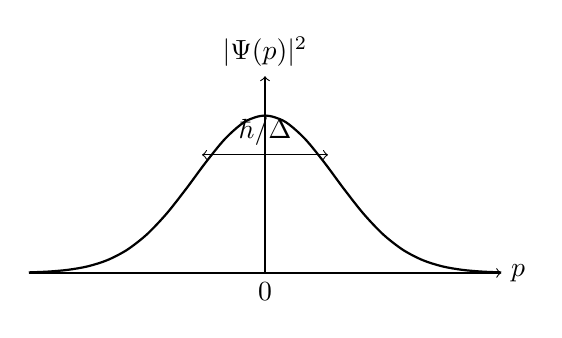
\begin{tikzpicture}[scale=1]
    \draw[->] (-3,0) -- (3,0) node[right] {$p$};
    \draw[->] (0,0) -- (0,2.5) node[above] {$|\Psi(p)|^2$};
    \draw[scale=1, domain=-3:3, smooth, variable=\x, thick] plot ({\x},{2*exp(-(\x*\x)/1.6)});
    \draw[<->] (-0.8,1.5) -- (0.8,1.5) node[midway,above] {$\hbar/\Delta$};
    \node[below] at (0,0) {$0$};
\end{tikzpicture}
\end{center}

Trata-se de uma Gaussiana (como $|\Psi(x)|^2$) centrada em $p=0$, de largura $\dfrac{\hbar}{\Delta}$.

\subsection*{Transformada de Fourier de Gaussianas}

\begin{equation}
    \int_{-\infty}^{\infty} dx\; e^{-ikx}\, e^{-\alpha x^2} = \int_{-\infty}^{\infty} e^{-\alpha\left(x+\frac{ik}{2\alpha}\right)^2}\, e^{-k^2/4\alpha}\, dx
\label{eq:aula12_fourier_gaussiana_1}
\end{equation}

Esse procedimento, que se aplica quando você tem $\int e^{f(x)}\,dx$ e $f(x)$ é uma função \textbf{QUADRÁTICA} de $x$, se chama "completar os quadrados".

\begin{equation}
    = \sqrt{\frac{\pi}{\alpha}}\; e^{-k^2/4\alpha}
\label{eq:aula12_fourier_gaussiana_2}
\end{equation}
onde se usou que $\displaystyle\int_{-\infty}^{\infty} e^{-\alpha(x+x_0)^2}\,dx = \sqrt{\frac{\pi}{\alpha}}$ (mesmo que $x_0$ seja complexo!).

\textbf{TESTE DIMENSIONAL:} A integral acima deve ter dimensão $[x]$. Do argumento das exponenciais, $k = [x]^{-1}$ e $\alpha = [x]^{-2}$. No argumento da exponencial final temos
\begin{equation}
    \frac{k^2}{\alpha} = \frac{[x]^{-2}}{[x]^{-2}} = 1 \qquad \text{OK}
\label{eq:aula12_teste_dimensional_1}
\end{equation}

Na frente da exponencial temos
\begin{equation}
    \frac{1}{\sqrt{\alpha}} = \frac{1}{[x]^{-1}} = [x] \qquad \text{OK}
\label{eq:aula12_teste_dimensional_2}
\end{equation}

\fbox{\parbox{0.92\textwidth}{
Cheque \textbf{SEMPRE} se $\aver{R}$ e $\Delta R$ têm dimensão de $[R]$ e se $\aver{R^2}$ tem dimensão de $[R]^2$ (e se são \textbf{REAIS}).

\textbf{ERRO DIMENSIONAL NA PROVA SERÁ PUNIDO COM MORTE LENTA E DOLOROSA!}
}}
